\documentclass[a4paper,11pt]{article}
\usepackage[utf8]{inputenc}
\usepackage[french]{babel}
\usepackage[T1]{fontenc}
\usepackage{makeidx}
\makeindex
\usepackage{lmodern}
\usepackage{color}
\usepackage{graphicx}
\usepackage{listings}
\usepackage{caption}
\usepackage{subcaption}
 \usepackage{float}


\newcommand{\br}{\\\mbox{}}



\begin{document}

\pagenumbering{gobble}

\title{\color{red}Projet Génie Logiciel : \br\textbf{Gestion des services}}
\date{Décembre 2016}
\author{Sarra BOUTAHLIL\br Alexis DONNART}

\maketitle

\begin{abstract}
Dans le cadre du cours de génie logiciel de Master 1 ALMA 2016-2017 dispensé à l'Université de Nantes par S. Gerson, il nous à été demandé de concevoir et de mettre en œuvre un logiciel réparti permettant la gestion des services de différents enseignants.\br
L'objectif était d'effectuer l'analyse, la conception préliminaire ainsi que la conception détaillé du système afin de pouvoir le mettre en œuvre en Java.\br
\end{abstract}
\pagebreak

\tableofcontents


\pagebreak 
\section{Architecture}

\subsection{Introduction}

Dans un premier temps, nous nous attacherons à la description générale de l'architecture du système. Nous y présenterons les différentes vues (physique, logique, processus), ainsi que les réponses aux exigences non-fonctionnels.


\subsection{Vue physique}
La vue physique nous montre comment se comportera physiquement le système. La figure [\ref{DD}] présente le diagramme de déploiement du système basé sur deux grands composants matériels : le département et le client. Le département comportera la version de l'application prévue pour le chef de département, avec la persistance de données assurée. Le client lui sera conçu pour l'enseignant qui viendra utiliser un poste du département.\br
\begin{figure}[h]
\centering
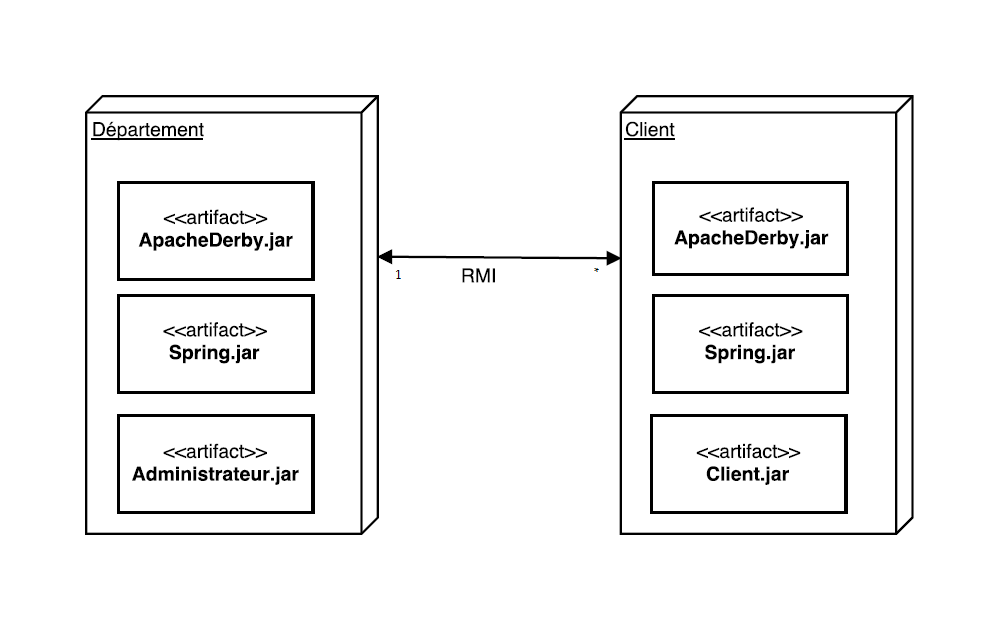
\includegraphics[scale=0.4]{Deploiment.png}
\caption{Diagramme de déploiement}
\label{DD}
\end{figure}
La figure [\ref{DDI}] représente un exemple de déploiement du système, composé de plusieurs départements, et plusieurs clients.\br
Nous déploierons sur chaque département et client un ensemble d'outils pour répondre aux exigences non-fonctionnelles correspondants aux artefacts.
\begin{figure}
\centering
\includegraphics[scale=0.4]{DDI.png}
\caption{Diagramme de déploiement d'instance}
\label{DDI}
\end{figure}

\subsection{Vue logique}
Nous nous intéressons à présent à un niveau plus détaillé : les paquetages UML. L'application sera décomposée en quatre grand paquetages [\ref{DP}], répondant chacun à une problématique. Le paquetage \textit{Départements} regroupe les fonctionnalités propres aux département, à savoir la gestion par le chef de département, la gestion du serveur distant, et la persistance. Le \textit{Client} de son côté gère tout les accès par le client au serveur ainsi que le stockage locale des données. Le paquetage \textit{Service} offre les accès du client aux données et requêtes sur le département. Tous se basent sur les données du paquetage \textit{Gestion de données}, décrivant le diagramme de classe de l'application.
\begin{figure}
\centering
\includegraphics[scale=0.5]{DP.png}
\caption{Diagramme de paquetage}
\label{DP}
\end{figure}


\subsection{Vue de processus}
Le déroulement de l'application se base sur deux(ou plusieurs) processus parallèles correspondant aux départements et aux clients. Chaque processus aura un rôle précis dans le système : enseignant (emettre des voeux, etc.) ou chef de département (validation des voeux, etc.). Tout ces processus se recoupent dans un but : la gestion des services des enseignants [\ref{Det}].
\begin{figure}
\centering
\includegraphics[scale=0.35]{DET.png}
\caption{Diagramme d'état transition global}
\label{Det}
\end{figure}
\subsection{Vue de fiabilité}
Pour assurer la fiabilité du système, sa maintenabilité ainsi que son interopérabilité, nous utiliserons le framework \textit{Spring}, permettant un développement et une maintenance facile. De plus ce framework permet la configuration simple de l'application, quelque soit la machine (utilisant la machine virtuelle java). Tout ces facteurs renforcent la fiabilité.
\subsection{Réponses aux exigences non-fonctionnelles}
Pour répondre aux exigences non-fonctionnelles, certains choix techniques se sont imposés.
\subsubsection{Gestion de la concurrence}
Pour assurer le bon fonctionnement du département et des clients en simultanés, nous avons choisi d'assurer la concurrence à l'aide d'un serveur \textit{Spring RMI}. Chaque département possèdera son serveur, assurant que chaque enseignant pourra s'y connecter.\br
En plus de répondre à des questions de maintenabilité du code, RMI offre un développement concurrent très rapide.
\subsubsection{Gestion de la persistance}
En plus de pouvoir se connecter à distance sur le serveur du département, nous souhaitions pouvoir stocker nos données de façon persistante. Pour se faire, nous avons utilisé \textit{Hibernate}, déployé sur le serveur du département. L'utilisateur client qui voudra stocker ses données devra le faire par le biais du serveur RMI à l'aide des \textit{repositories}. De même que pour la concurrence, le choix de Hibernate s'est axé sur la simplicité d'utilisation et la facilité de maintenabilité du code.
\subsubsection{Gestion de la sécurité}
La sécurité est remise aux implémentations faites de Spring RMI et de Hibernate, aucune sécurité supplémentaire n'a été mise en place.
\subsection{Architecture technique : traduction de UML en code source}
Pour traduire la conception et l'architecture développé, nous avons établis des règles de base pour la traduction.
\subsubsection{Règles de traduction des types de base}
Pour traduire les types de base (Hour, TypeEnseignement), nous utiliserons des classes regroupant les informations nécessaires au type de base.
\subsubsection{Règles de traduction des classes}
Plusieurs règles s'appliquent pour les classes : toutes les classes UML deviennent des classes java, pas d'interface. Tous les attributs seront annotés à l'aide de hibernate pour respecter les relations. De même, si des instances sont nécessaires, ils seront injectés à l'aide de Spring.
\subsubsection{Règles de traduction des associations, agrégations composites et agrégations partagées}
Pour traduire les relations, nous avons respecter ces principes :\br
\begin{itemize}
\item 1 Une relation 1 à n : Une liste pour représenter les n éléments, un attribut pour représenter le 1. 
\item 2 Une relation 1 à 1 : Une référence unidirectionnelle dans les deux sens, d'un objet à un objet.
\item 3 Une relation n à n : Une liste des deux côtés pour représenter le lien bidirectionnel.
\end{itemize}
Dans tous les cas, nous prêtons attention aux problèmes d'intégrité référentielles.

\subsection{Patrons architecturaux utilisés}
Plusieurs patrons de conceptions pouvaient faciliter la conception de l'application.
\subsubsection{Patron Façade}
Notre système doit offrir une interface simple et clair pour l'utilisateur. Bien que simple d'utilisation, l'ajout de la persistance et de la concurrence complexifie la lisibilité pour l'utilisateur. Pour cibler les fonctionnalités de chaque partie, nous offrirons une \textit{Façade} pour la vue client et une pour la vue département, n'offrant que des fonctionnalités de haut niveau. C'est tout le principe de la façade : regrouper des éléments complexes pour n'en offrir qu'une version facilité.
\subsubsection{Patron Etat}
Notre système sera décomposé en plusieurs composants qui viendront réaliser certaines actions : émission d'une demande, publication d'une demande puis affectation d'une demande. Ce cycle reste valide pour toute la durée d'utilisation de l'application, on pourra donc représenter ce cycle par un patron état qui permettrait de passer d'un état à l'autre facilement.


\section{Spécification des composants}
\subsection{Introduction}
Nous allons décrire les composants de notre système et leur fonctionnement au sein de l'application. Nous décrirons certains cas d'utilisation de ces processus.

\subsection{Description des composants}
Notre système est décomposé en trois composants.
\subsubsection{Le composant Emission}
Le composant Emission [\ref{DSUC1}] offre les fonctionnalités nécessaires à la réalisation de l'émission d'un souhait pour l'enseignant. Ce composant se traduit par une interface proposant la fonctionnalité implémenté par une façade cachant le reste du système : l'utilisateur n'a ainsi accès qu'à l'unique fonctionnalité voulu : l'émission.
\begin{figure}[ht]
\centering
\includegraphics[scale=0.5]{ComposantA.png}
\caption{Composant : émission}
\label{DSUC1}
\end{figure}
\subsubsection{Le composant Publication}
Sur le même principe, le composant Publication [\ref{DSUC2}] offre une façade implémentant la fonction Publier, servant au chef de département à publier les voeux des enseignants.
\begin{figure}[ht]
\centering
\includegraphics[scale=0.5]{ComposantB.png}
\caption{Composant : publication}
\label{DSUC2}
\end{figure}
\subsubsection{Le composant Affectation}
Finalement, le composant Affectation [\ref{DSUC3}] offre la fonction Affecter au chef de département.
\begin{figure}[ht]
\centering
\includegraphics[scale=0.5]{ComposantC.png}
\caption{Composant : affectation}
\label{DSUC3}
\end{figure}
\subsection{Interactions}
Avec les composants du système décrit, il est important maintenant de comprendre les interactions entre ces composants, nous allons pour cela étudier des diagrammes de séquences décrivant chaque composant et chaque cas d'utilisation.
\subsubsection{Cas d’utilisation UC1}
Après avoir bien étudié les scénarios du cas d'utilisation d'affectation des souhaits, nous obtenons trois cas possibles, comprenant un cas nominal et deux cas extra nominaux.
\textbf{Le cas nominal}
Le chef de département souhaite ici [\ref{DUC1}] récupérer la liste des voeux des enseignants pour pouvoir leur affecter des enseignements. Dans ce cas, le chef de département suit les vœux des enseignants. Une intervention au département sera créé.\br
\begin{figure}
\centering
\includegraphics[scale=0.4]{SeqUC1.png}
\caption{Diagramme de Séquence UC1: cas nominal}
\label{DUC1}
\end{figure}
Dans un premier cas extra-nominal [\ref{DUC1_}], il s'agit d'affecter une demande extérieur suivant les souhaits d'un enseignant.
\begin{figure}

\centering
\includegraphics[scale=0.4]{SeqUC1_.png}
\caption{Diagramme de séquence UC1: cas extra nominal 1}
\label{DUC1_}
\end{figure}

Dans un dernier cas [\ref{DUC1__}], le chef du département, après avoir récupéré la liste des enseignants, impose une intervention à un enseignant.
\begin{figure}
\centering
\includegraphics[scale=0.4]{Seq_UC1.png}
\caption{Diagramme de séquence UC1: cas extra nominal 2}
\label{DUC1__}
\end{figure}

\subsubsection{Cas d’utilisation UC2}
Dans ce deuxième cas d'utilisation [\ref{DUC2}], le chef de département visualise les demandes des enseignants. Une fois visualisés, il peut choisir d'en valider : les rendre publique aux autres enseignants.
\begin{figure}
\centering
\includegraphics[scale=0.5]{Seq_UC2.png}
\caption{Diagramme de séquence UC2: cas nominal}
\label{DUC2}
\end{figure}
\subsubsection{Cas d’utilisation UC3}
Dans le troisième cas d'utilisation [\ref{DUC3}], le chef du département visualise la liste des demandes publiés puis vient corriger les affectations des enseignants. Si un enseignant a été affecté par erreur à une intervention, le chef de département pourra le changer.
\begin{figure}
\centering
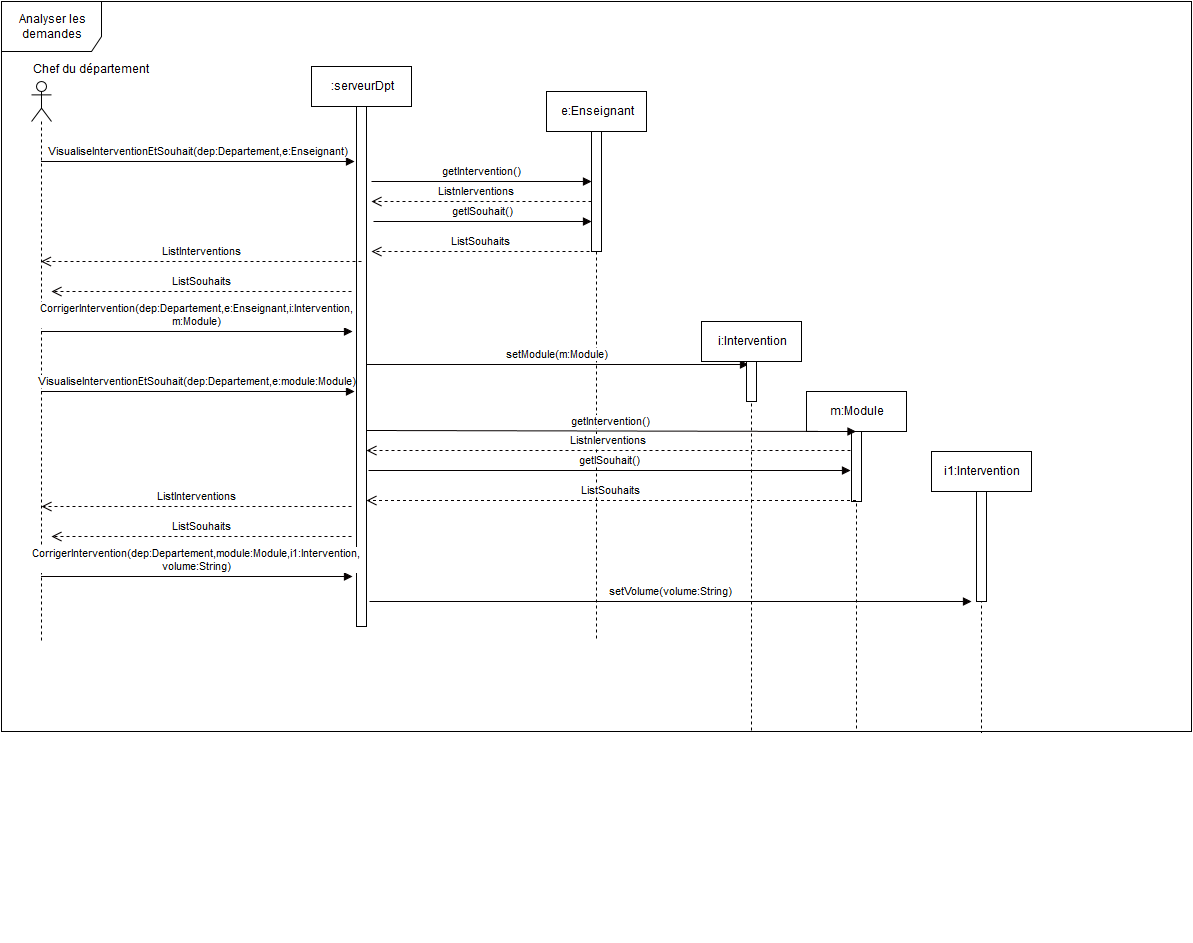
\includegraphics[scale=0.4]{Seq_UC3.png}
\caption{Diagramme de séquence UC3: cas nominal}
\label{DUC3}
\end{figure}

\subsubsection{Cas d’utilisation UC4}
L'enseignant pourra émettre une liste de vœux [\ref{DUC4}] vers le département pour la rendre permanente. Les vœux ne seront publiques au reste des enseignants que si le chef de département les rends publiques [UC \ref{DUC2}].\br
\begin{figure}
\centering
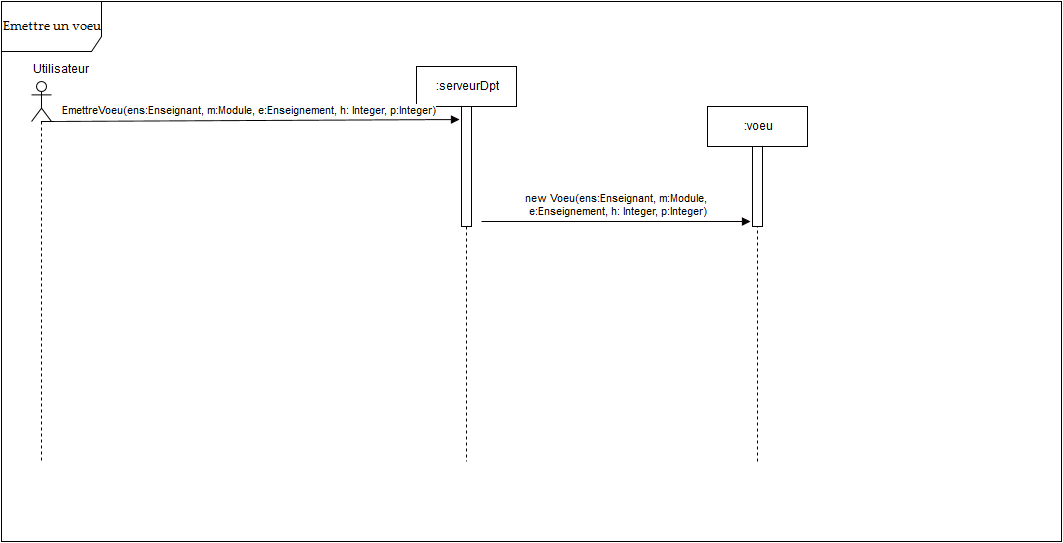
\includegraphics[scale=0.5]{Seq_UC4.png}
\caption{Diagramme de séquence UC4: cas nominal}
\label{DUC4}
\end{figure}
Le premier cas alternatif [\ref{DUC4_}] correspond à l'émission d'une liste de demande extérieur.\br
\begin{figure}
\centering
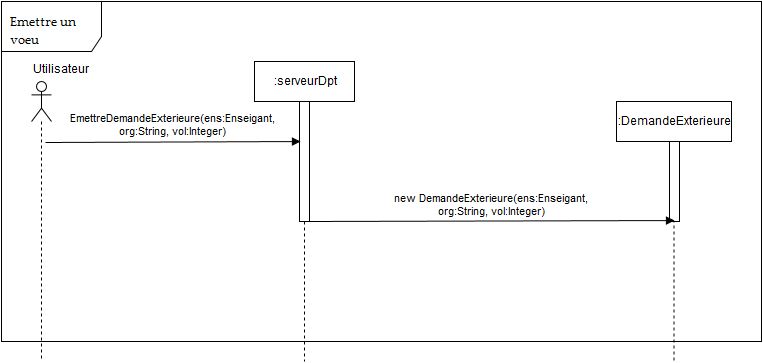
\includegraphics[scale=0.5]{Seq_UC4_.png}
\caption{Diagramme de séquence UC4: cas extra nominal 1}
\label{DUC4_}
\end{figure}
Le deuxième cas alternatif [\ref{DUC4__}] correspond à l'émission d'une liste de demande spéciale.\br
\begin{figure}
\centering
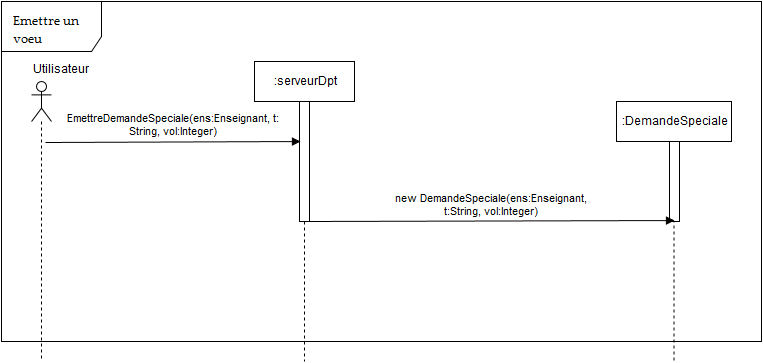
\includegraphics[scale=0.5]{Seq_UC4__.png}
\caption{Diagramme de séquence UC4: cas extra nominal 2}
\label{DUC4__}
\end{figure}
Le dernier cas alternatif [\ref{DUC4___}] correspond à l'émission d'une liste de vœux avec détection de conflit. Lors de l'émission, l'enseignant sera prévenu à l'aide d'une exception du ou des vœux qui sont en conflit pour le corriger en local.
\begin{figure}
\centering
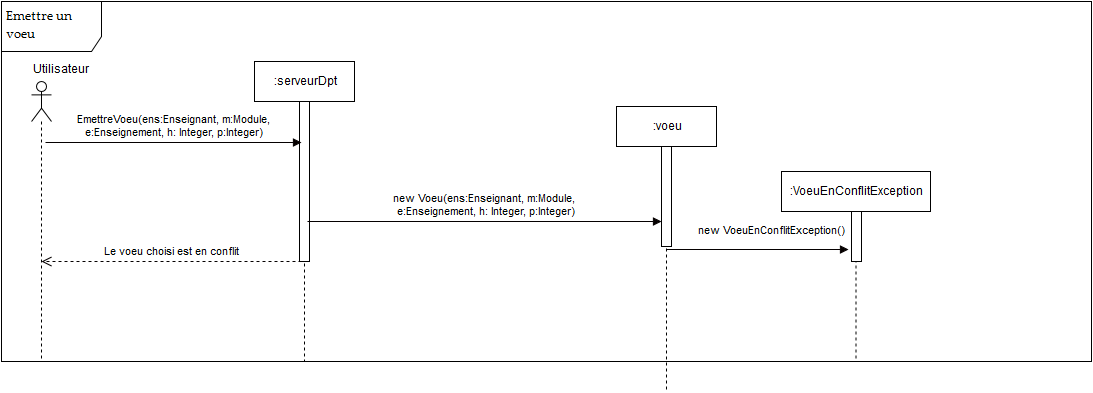
\includegraphics[scale=0.5]{Seq_UC4___.png}
\caption{Diagramme de séquence UC4: cas extra nominal 3}
\label{DUC4___}
\end{figure}

\subsubsection{Cas d’utilisation UC5}
L'enseignant pourra transmettre au chef de département une liste de voeux préalablement sélectionnée [\ref{DUC5}]. Ce dernier pourra alors publier la liste.\br
\begin{figure}
\centering
\includegraphics[scale=0.5]{Seq_UC5.png}
\caption{Diagramme de séquence UC5: cas nominal}
\label{DUC5}
\end{figure}
Le premier cas alternatif [\ref{DUC5_}] correspond à l'annulation d'une liste de souhait transmise : le chef de département n'en tiendra pas compte.\br
\begin{figure}
\centering
\includegraphics[scale=0.5]{Seq_UC5_.png}
\caption{Diagramme de séquence UC5: cas nominal extra nominal 1}
\label{DUC5_}
\end{figure}
Le deuxième cas alternatif [\ref{DUC5__}] correspond à l'émission d'une liste de voeux, mais les voeux ont déjà été affectés ou ont été supprimés.\br
\begin{figure}
\centering
\includegraphics[scale=0.5]{Seq_UC5__.png}
\caption{Diagramme de séquence UC5: cas nominal extra nominal21}
\label{DUC5__}
\end{figure}
Le dernier cas alternatif [\ref{DUC5___}] correspond à l'émission d'une liste de voeux, mais la liste est vide, une exception \textit{PasDeVoeuEnAttente} est renvoyé pour notifier l'enseignant.\br
\begin{figure}
\centering
\includegraphics[scale=0.5]{Seq_UC5___.png}
\caption{Diagramme de séquence UC5: cas nominal extra nominal 3}
\label{DUC5___}
\end{figure}

\subsubsection{Cas d’utilisation UC6}
Le dernier cas d'utilisation [\ref{DUC6}] permet a un enseignant de consulter la liste des enseignements disponibles avant d'effectuer ses voeux.
\begin{figure}
\centering
\includegraphics[scale=0.5]{Seq_UC6.png}
\caption{Diagramme de séquence UC6: cas nominal}
\label{DUC6}
\end{figure}

\subsection{Spécification des interfaces}
Pour chaque composant, on disposera d'une interface implémentant les fonctions de base.
\subsubsection{Interface IEmissionSouhait}
Le composant \textit{Emission} implémente l'interface IEmissionSouhait décrivant la méthode \textit{Emettre(Enseignant, Demande, Département)}. Cette fonction implémentera l'émission d'une demande d'un enseignant appartenant à un département vers le serveur de ce département par cet enseignant.
\subsubsection{Interface IPublicationSouhait}
Le composant \textit{Publier} implémente l'interface IPublicationSouhait décrivant la méthode \textit{Publier(Département, List<Demande>)}. Cette fonction implémentera la publication d'une liste de demandes d'un enseignant appartenant à un département sur le serveur de ce département par le chef de ce département.
\subsubsection{Interface IAffectationSouhait}
Le composant \textit{Affecter} implémente l'interface IAffectationSouhait décrivant la méthode \textit{Affecter(Département, Demande, Enseignant)}. Cette fonction implémentera l'affectation d'une demande d'un enseignant appartenant à un département sur le serveur de ce département par le chef de ce département
\subsection{Spécification des types utilisés}
Pour décrire l'application, les types ont été divisés en plusieurs catégories.
\subsubsection{Données}
Un type a été utilisé pour chaque classe de données (\textbf{Enseignant}, \textbf{Demande}, \textbf{Département}, etc). Ces classes ont pour attributs ceux spécifiés par le diagramme UML. Chaque attribut a été annoté pour l'utilisation.
\subsubsection{Service}
Pour l'utilisation combiné de Spring RMI et de Hibernate, nous avions besoin d'un type pour gérer la communication : 
\begin{itemize}
\item \textbf{Service} : contient les Repositories Hibernate en tant qu'attributs, et offre les méthodes d'accès via Spring RMI pour le client.
\end{itemize}
\subsubsection{Département}
Le département contient les classes qui seront utilisés par le serveur du département pour gérer la persistance des données ainsi que le serveur.
\begin{itemize}
\item \textbf{Persistance} : toutes les classes de Repository Hibernate, contenant chaque les accès aux données persistantes.
\item \textbf{Serveur} : classe de lancement du serveur du département.
\end{itemize}

\section{Conception détaillée}
\subsection{Introduction}
Après avoir effectué l'analyse puis la conception préliminaire, nous avons suffisamment d'éléments pour la conception détaillé. Nous tâcherons de décrire le comportement détaillé des composants ainsi que des choix de conception.
\subsection{Répertoire des décisions de conception}
Nous avons évoqué plus tôt des patrons pour concevoir notre système, revenons sur l'implémentation.

\subsubsection{Patron Façade}
Le patron de conception façade est utilisé pour offrir à l'utilisateur (enseignant ou chef de département) les fonctions utiles à son utilisation.\br
Chaque composant (Publication, Emission, Affectation) possède sa façade, offrant un ensemble de fonction utile à la réalisation de la tâche prévu. Cette façade masque l'utilisation du \textbf{Service} pour communiquer avec Spring RMI. Des fonctions d'ajout, de suppression et de mise à jour des données sont disponibles point de vue chef de département (Publication et affectation). Pour l'enseignant (Emission), seul les fonctions d'émission et d'authentification sont disponibles.

\subsection{Spécification détaillée des composants}
Détaillons maintenant les composants implémentés.

\subsubsection{Composant Emission}

\subsubsection*{Structure}
Le composant Emission[\ref{DAE__}] sera présenté par la façade masquant l'utilisation des classes de données et des fonctionnalités de Spring/Hibernate. Cette façade implémente l'interface IEmissionSouhait offrant la fonction Emission à l'enseignant.
\begin{figure}
\centering
\includegraphics[scale=0.3]{DC-ComposantA.png}
\caption{Diagramme de classe du composant Emettre}
\label{DAE__}
\end{figure}

\subsubsection*{Comportement}

Le comportement interne du composant Emission est décrit à l'aide des diagrammes état-transition [\ref{DAE}] et d'activité [\ref{DAE_}].\br
Le comportement implémente toutes les situations décrites par ses cas d'utilisations.

\begin{figure}
\centering
\includegraphics[scale=0.3]{ComposantAEtat.png}
\caption{Diagramme état transition du composant Emission}
\label{DAE}
\end{figure}

\begin{figure}
\centering
\includegraphics[scale=0.3]{ActiviteComposantA.png}
\caption{Diagramme d'activité de l'opération Emettre}
\label{DAE_}
\end{figure}






\subsubsection{Composant Publication}
\subsubsection*{Structure}
Le composant Publication[\ref{DBE__}] sera également présenté par sa façade, masquant l'utilisation des classes de données. Cette façade implémente l'interface IPublicationSouhait offrant la fonction Publier au chef du département.

\begin{figure}
\centering
\includegraphics[scale=0.3]{DC-ComposantB.png}
\caption{Diagramme de classe du composant Pulication}
\label{DBE__}
\end{figure}

\subsubsection*{Comportement}
Le comportement interne du composant Publication est décrit à l'aide des diagrammes état-transition [\ref{DBE}] et d'activité [\ref{DBE_}].\br
Le comportement implémente toutes les situations décrites par ses cas d'utilisations.
\begin{figure}
\centering
\includegraphics[scale=0.3]{ComposantBEtat.png}
\caption{Diagramme état transition du composant Publication}
\label{DBE}
\end{figure}

\begin{figure}
\centering
\includegraphics[scale=0.3]{ActiviteComposantB.png}
\caption{Diagramme d'activité de l'opération Publier}
\label{DBE__}
\end{figure}

\subsubsection{Composant Affectation}
\subsubsection*{Structure}
Finalement, le composant Affectation[\ref{DCE__}], sur le même principe sera présenté par sa façade. Cette façade implémente l'interface IAffectationSouhait offrant la fonction Affecter au chef du département.
\begin{figure}
\centering
\includegraphics[scale=0.3]{DC-ComposantC.png}
\caption{Diagramme de classe du composant Affectation}
\label{DCE__}
\end{figure}

\subsubsection*{Comportement}
Le comportement interne du composant Affectation est décrit à l'aide des diagrammes état-transition [\ref{DCE}] et d'activité [\ref{DCE_}].\br
Le comportement implémente toutes les situations décrites par ses cas d'utilisations.
\begin{figure}
\centering
\includegraphics[scale=0.3]{ComposantCEtat.png}
\caption{Diagramme état transition du composant Affectation}
\label{DCE}
\end{figure}

\begin{figure}
\centering
\includegraphics[scale=0.3]{ActiviteComposantC.png}
\caption{Diagramme d'activité de l'opération Affecter}
\label{DCE_}
\end{figure}






\pagebreak 
\end{document}
